\subsection{Search Space}

Der Suchraum (Search Space) bildet die Grundlage für die Suche nach einem optimalen Plan. Innerhalb des Suchraums findet die Auswahl des optimalen Plans statt. 
Zuerst wird der Search Space erforscht. In einem zweiten Schritt werden die alternativen Pläne bewertet. Am Ende wird der optimale Plan ausgeführt.



Als Search Space wird die Menge der logisch äquivalenten Pläne, die auf Grund einer Anfrage gebildet werden können, bezeichnet. Die Menge der äquivalenten Pläne kann so mächtig und so groß sein, dass nicht alle äquivalenten Pläne mit Hilfe von bekannten Techniken gefunden werden können. Bei einigen Systemen ist es möglich, dass die Suche vorab abgebrochen wird und so nicht alle Pläne gefunden werden können. Der Search Space, der mit Hilfe dieser bekannten Mittel gefunden werden kann, wird als potenzieller Suchraum (Potential Search Space) bezeichnet. Die Pläne, die innerhalb dieses Search Spaces liegen, werden auf Grund ihrer Erreichbarkeit auch als accessable bezeichnet. Die Menge der Pläne, die nicht gefunden werden können, heißen folglich non-accessable. Da selbst die Menge der Pläne des Potential Search Spaces sehr groß sein kann, berechnen Anfrageoptimierer i.d.R. ihre Suche nach Planalternativen ab. Die Menge der tatsächlich gefundenen Alternativen wird als tatsächlicher Suchraum (Actual Search Space) bezeichnet.


\begin{figure}[ht]
  \centering
  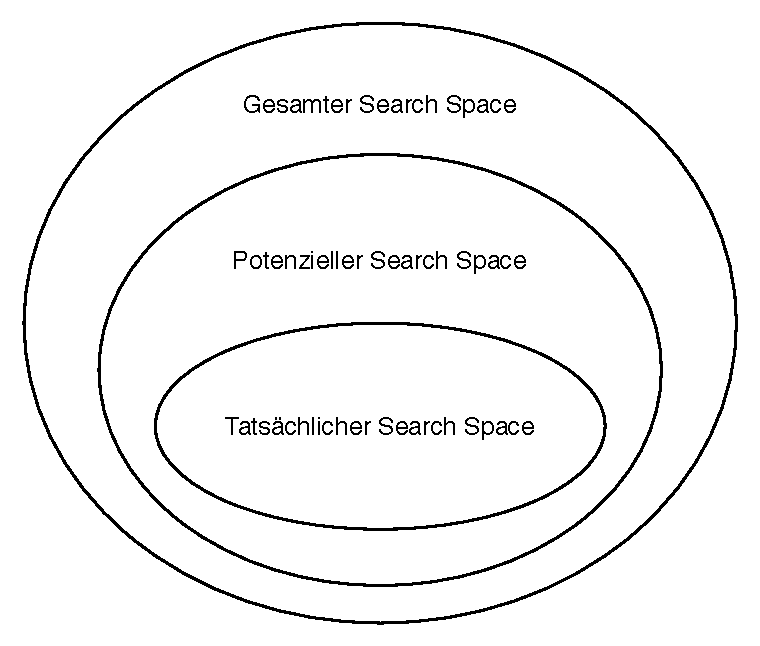
\includegraphics[scale=0.75]{02_Related_Work/SearchSpace.pdf}
  \caption{Search Space}
  \label{SearchSpace}
\end{figure}

In Abbildung \ref{SearchSpace} ist der optimale Fall eines Search Spaces zu sehen. Der Actual Search Space ist ein Subset des Potential Search Spaces und dieser wiederum ein Subset des gesamten Search Spaces. In der Realität sind auch andere Formen möglich. Dem actual Search Space können beispielsweise durch eine fehlerhafte Implementierung falsche Pläne zugeordnet werden.

Um einen Search Space zu erforschen,  kommen Enumeratoren zum Einsatz. Diese werden im nächsten Abschnitt genauer behandelt.